\begin{figure}[H]
\begin{center}
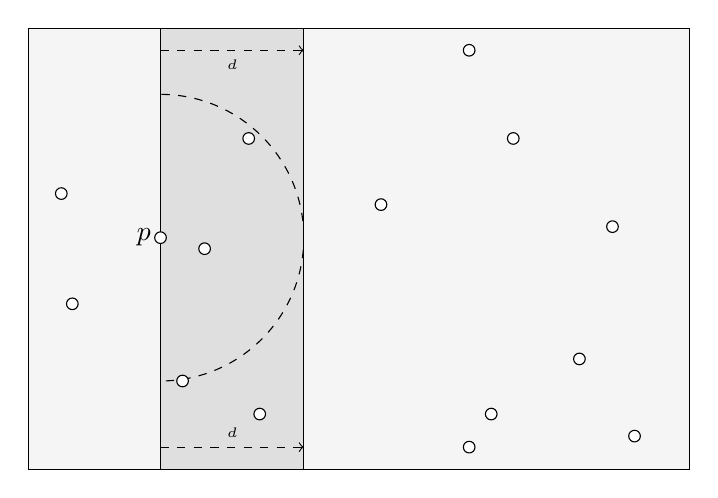
\begin{tikzpicture}[scale=1.4]
	\fill[lightgray!15,draw=black] (0,0) rectangle (6,4);
	\fill[lightgray!50,draw=black] (1.2,0) rectangle (2.5,4);
	\begin{scope}
	\clip (1.2,0) rectangle (2.5,4);
	\draw[dashed](1.2,2.1) circle (1.3);
	\end{scope}
	
	\draw [dashed,->](1.2,0.2) -- node[above]{\tiny$d$}(2.5,0.2);

	\draw [dashed,->](1.2,3.8) -- node[below]{\tiny$d$}(2.5,3.8);

	\node[left] at (1.2,2.1) {$\tiny p$};

	\fill[white,draw=black] (3.2,2.4) circle (1.5pt);
	\fill[white,draw=black] (5,1) circle (1.5pt);		
	\fill[white,draw=black] (4.2,0.5) circle (1.5pt);
	\fill[white,draw=black] (4,0.2) circle (1.5pt);
	\fill[white,draw=black] (5.5,0.3) circle (1.5pt);
	\fill[white,draw=black] (4.4,3) circle (1.5pt);
	\fill[white,draw=black] (4,3.8) circle (1.5pt);
	\fill[white,draw=black] (5.3,2.2) circle (1.5pt);
	\fill[white,draw=black] (1.6,2) circle (1.5pt);
	\fill[white,draw=black] (1.2,2.1) circle (1.5pt);
	\fill[white,draw=black] (2,3) circle (1.5pt);
	\fill[white,draw=black] (0.3,2.5) circle (1.5pt);
	\fill[white,draw=black] (1.4,0.8) circle (1.5pt);
	\fill[white,draw=black] (2.1,0.5) circle (1.5pt);
	\fill[white,draw=black] (0.4,1.5) circle (1.5pt);

\end{tikzpicture}
\end{center}
\caption[Illustration of the Line Sweep method.]{Illustration of the Line Sweep method. This query searches for the points within a given distance of $p$ that are to the right of $p$}
\label{fig:ls1}
\end{figure}